% HIKET -- the storyline (live document; the basis for the story discussion, not a draft).
% Built on Lorenzo's decisions of 2026-10-12, story recomposed 2026-10-13 (for Samuli and Aleksi):
% general problem -> the Finnish case (forestry history, soil slowing: saturation?) -> the trilemma
% in Finland as a hypothesis; R1 the first test (balanced start fails); R2 the resolution (relaxed
% assumption works, the ridge shifts; S16 = the bridge); R3 forecasts, "did we get it wrong?", with
% two side arcs (temperature sensitivity; inputs and saturation); R4 future development, the
% speculative side arc (Discussion folded in); conclusions: saturation / limits / forecasts / plots.
% Numbers (restated 2026-10-13): production 20261012_1042*, balanced start 20261012_12*-13* -- both with
% the 1961-1984 pre-run climate (jobs 2227219-24 and 2234048-53).
\documentclass[11pt]{article}
\usepackage[utf8]{inputenc}\usepackage[T1]{fontenc}
\usepackage[margin=2.4cm]{geometry}
\usepackage{graphicx}\usepackage{amsmath}\usepackage{amssymb}\usepackage{xcolor}
\usepackage{float}\usepackage[hidelinks]{hyperref}
\usepackage{caption}\captionsetup{font=small,labelfont=bf}
\usepackage[most]{tcolorbox}
\usepackage{tikz}\usetikzlibrary{positioning, arrows.meta, calc, fit, backgrounds}
\usepackage{titlesec}\usepackage{placeins}
\titlespacing*{\paragraph}{0pt}{0.9\baselineskip}{0.4em}
\setcounter{secnumdepth}{4}\setcounter{tocdepth}{2}

% --- STRUCTURAL TOGGLE ---------------------------------------------------
% \combinedtrue  = one "Results and Discussion" section (recommended, and what
%                  Lorenzo leaned toward). \combinedfalse = classic split.
% Nothing else changes; the same blocks are emitted either way.
\newif\ifcombined \combinedtrue

\definecolor{notebg}{HTML}{EAF2FB}\definecolor{noterule}{HTML}{2C6FB5}
\newtcolorbox{note}{colback=notebg, colframe=noterule, boxrule=0pt, leftrule=3pt,
  arc=1pt, left=8pt, right=8pt, top=5pt, bottom=5pt, fontupper=\small,
  before skip=7pt, after skip=7pt}
\definecolor{testbg}{HTML}{EAF7EE}\definecolor{testrule}{HTML}{2E8B57}
\newtcolorbox{test}{colback=testbg, colframe=testrule, boxrule=0pt, leftrule=3pt,
  arc=1pt, left=8pt, right=8pt, top=5pt, bottom=5pt, fontupper=\small,
  before skip=7pt, after skip=7pt}
\definecolor{warnbg}{HTML}{FDF3E3}\definecolor{warnrule}{HTML}{C08A2E}
\newtcolorbox{warn}{colback=warnbg, colframe=warnrule, boxrule=0pt, leftrule=3pt,
  arc=1pt, left=8pt, right=8pt, top=5pt, bottom=5pt, fontupper=\small,
  before skip=7pt, after skip=7pt}
\definecolor{lorbg}{HTML}{F3EDF9}\definecolor{lorrule}{HTML}{6B3FA0}
\newtcolorbox{ann}{colback=lorbg, colframe=lorrule, boxrule=0pt, leftrule=3pt,
  arc=1pt, left=8pt, right=8pt, top=5pt, bottom=5pt, fontupper=\small,
  before skip=7pt, after skip=7pt}

\newcommand{\sinit}{\sigma_{\mathrm{init}}}
\newcommand{\sinput}{\sigma_{\mathrm{input}}}

% --- figure embedding (same machinery as v2) -----------------------------
\graphicspath{{figures/}{../Reporting/NextgenC_report/SOC_maps/thumbnails/}}
\newcommand{\FIGlabel}[1]{\textcolor{noterule}{\small$\blacktriangleright$ \textsf{#1}}}
\newcommand{\FIG}{\begingroup\catcode`\_=12\relax\FIGaux}
\newcommand{\FIGaux}[1]{%
  \FIGlabel{#1}\endgroup
  \IfFileExists{figures/#1.png}{%
    \begin{figure}[htbp]\centering
      \includegraphics[width=0.92\linewidth,height=0.40\textheight,keepaspectratio]{figures/#1.png}
      \caption{\textsf{#1}}\end{figure}}{%
  \IfFileExists{figures/#1.tex}{%
    \begin{table}[htbp]\centering\scriptsize\input{figures/#1.tex}\end{table}}{%
  \IfFileExists{../Reporting/NextgenC_report/SOC_maps/thumbnails/#1.png}{%
    \begin{figure}[htbp]\centering
      \includegraphics[width=0.58\linewidth,height=0.42\textheight,keepaspectratio]{#1.png}
      \caption{\textsf{#1} (NextGenC deliverable)}\end{figure}}{%
  \textcolor{warnrule}{\small[\textsf{#1} --- FILE NOT FOUND]}}}}}
% \FIGX cites a figure without embedding it. Needs the same catcode dance as \FIG,
% or an underscore in the name is read as a subscript and the build dies.
\newcommand{\FIGX}{\begingroup\catcode`\_=12\relax\FIGXaux}
\newcommand{\FIGXaux}[1]{\FIGlabel{#1}\endgroup}
\newcommand{\NEW}[1]{\textcolor{testrule}{\small$\bigstar$ \textsf{TO BUILD: #1}}}
\newcommand{\LIT}[1]{\textcolor{lorrule}{\small$\Box$ \textsf{LIT REVIEW: #1}}}

% --- REFERENCE ANNOTATION (added 2026-09-04) ------------------------------
% Every core claim carries the sources it rests on, in one short line under the
% paragraph. \vd = quote/number verified against the source; \nd = still to check.
% Full evidence tables and draft text: literature/NN_topic/README.md.
\definecolor{refrule}{HTML}{45566B}
\newcommand{\vd}{\textcolor{testrule}{$\checkmark$}}
\newcommand{\nd}{\textcolor{lorrule}{$\square$}}
% --- RESULT / DISCUSSION NESTING (added 2026-09-04) ------------------------
% Combined Results and Discussion, nested at SUBSECTION level: each subsection
% gives its result, then its interpretation, as SEPARATE paragraphs. \dparagraph
% marks the interpretation half so the rhythm is visible at a glance and the two
% halves stay mechanically separable if a journal demands the classic split.
\newcommand{\dparagraph}[1]{\paragraph{\textcolor{noterule}{$\rightsquigarrow$}\ #1}}
\newcommand{\refs}[1]{\par\vspace{-0.25em}{\footnotesize\color{refrule}%
  \hangindent=1.3em\hangafter=1 $\vdash$~\textsc{refs}\,\ #1\par}\vspace{0.15em}}

% --- INLINE FIGURES (2026-10-12): placed where they are used ([H], no floating), caption tagged.
%   \FIG  main text   \FIGA  appendix   \FIGQ  not in Lorenzo's list (keep?)
\newcommand{\FIGshow}[2]{\FIGlabel{#1}\endgroup
  \IfFileExists{figures/#1.png}{%
    \begin{figure}[H]\centering
      \includegraphics[width=0.86\linewidth,height=0.36\textheight,keepaspectratio]{figures/#1.png}
      \caption{\textsf{#1}#2}\end{figure}}{\textcolor{warnrule}{\small[\textsf{#1} --- FILE NOT FOUND]}}}
\renewcommand{\FIGaux}[1]{\FIGshow{#1}{ --- main text}}
\newcommand{\FIGA}{\begingroup\catcode`\_=12\relax\FIGAaux}
\newcommand{\FIGAaux}[1]{\FIGshow{#1}{ --- \textcolor{warnrule}{\textbf{appendix}}}}
\newcommand{\FIGQ}{\begingroup\catcode`\_=12\relax\FIGQaux}
\newcommand{\FIGQaux}[1]{\FIGshow{#1}{ --- \textcolor{lorrule}{\textbf{not in your list: keep?}}}}


% =====================================================================
% ARC SCHEMAS. One per section, nested: each opens with the strip of the whole paper,
% its own section highlighted, then the section's internal arc.
% cl = claim; key = the section's payload; cav = caveat that travels with a claim;
% thr = a thread of the trilemma coming back; ev = evidence line under a claim.
% =====================================================================
\tikzset{
  cl/.style={rectangle, rounded corners=2pt, draw=black!45, fill=white, align=left,
             inner sep=3pt, font=\scriptsize, text width=#1},
  cl/.default=46mm,
  key/.style={draw=blue!55!black, fill=blue!8, thick},
  thr/.style={draw=violet!70!black, fill=violet!6, thick},
  cav/.style={draw=warnrule, fill=warnbg, font=\tiny},
  arr/.style={-{Latex[length=1.8mm]}, thick, black!55},
  arrk/.style={-{Latex[length=2.1mm]}, very thick, blue!50!black},
  arrt/.style={-{Latex[length=2.1mm]}, very thick, violet!60!black, dashed},
  grp/.style={rectangle, rounded corners=3pt, draw=black!25, fill=black!3, inner sep=5pt},
  glab/.style={font=\tiny\scshape, text=black!60, anchor=south west, inner sep=1pt}
}
\newcommand{\ev}[1]{\\[-1pt]{\tiny\itshape\color{black!60}#1}}
\newcommand{\gapnote}[1]{\textcolor{warnrule}{\textbf{[OPEN:} #1\textbf{]}}}
\newcommand{\TR}{{\tiny\bfseries\color{violet!70!black}[trilemma]}}

% --- the strip of the whole paper, section #1 highlighted (1..7) ---
\newcommand{\archstrip}[1]{%
\begin{center}
\begin{tikzpicture}[font=\tiny,
  sb/.style={rectangle, rounded corners=1pt, draw=black!35, fill=black!4, minimum height=5mm,
             text width=19mm, align=center, inner sep=1pt},
  hb/.style={sb, draw=noterule, fill=notebg, very thick, font=\tiny\bfseries}]
\foreach \t [count=\k] in {Introduction, Methods, {R1\\the problem}, {R2\\the resolution},
                           {R3\\forecasts}, {R4\\future development}, Conclusions} {
  \ifnum\k=#1 \node[hb] (s\k) at ({(\k-1)*2.33}, 0) {\t};
  \else       \node[sb] (s\k) at ({(\k-1)*2.33}, 0) {\t}; \fi
}
\foreach \k [evaluate=\k as \j using int(\k+1)] in {1,...,6} \draw[-{Latex[length=1.2mm]}, black!40] (s\k) -- (s\j);
\end{tikzpicture}
\end{center}\vspace{-0.6em}}
\newcommand{\arch}[2]{\par\noindent\begin{minipage}{\linewidth}\archstrip{#1}#2\end{minipage}\par\medskip}

% --- OVERALL ---
\newcommand{\archOverall}{%
\begin{center}
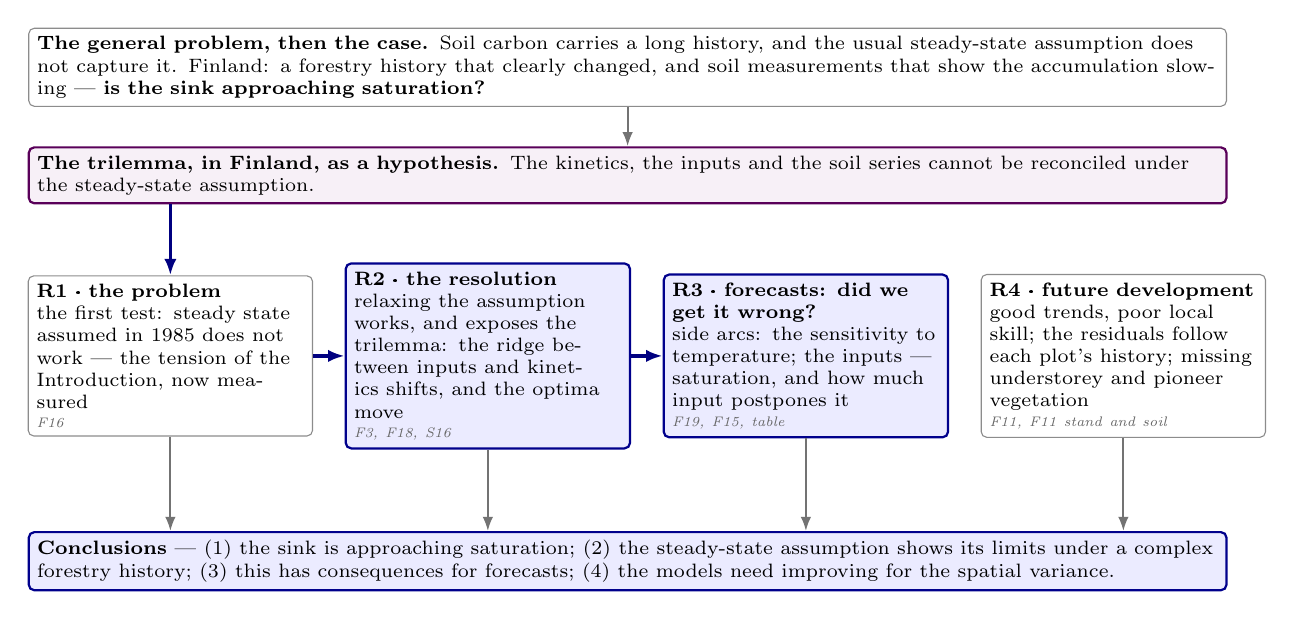
\begin{tikzpicture}[node distance=5mm]
\node[cl=150mm] (G) {\textbf{The general problem, then the case.} Soil carbon carries a long history, and the
  usual steady-state assumption does not capture it. Finland: a forestry history that clearly changed, and soil
  measurements that show the accumulation slowing --- \textbf{is the sink approaching saturation?}};
\node[cl=150mm, thr, below=of G] (T) {\textbf{The trilemma, in Finland, as a hypothesis.} The kinetics, the
  inputs and the soil series cannot be reconciled under the steady-state assumption.};
\node[cl=34mm, below=9mm of T.south west, anchor=north west] (R1) {\textbf{R1 · the problem}\\the first test:
  steady state assumed in 1985 does not work --- the tension of the Introduction, now measured \ev{F16}};
\node[cl=34mm, key, right=4mm of R1] (R2) {\textbf{R2 · the resolution}\\relaxing the assumption works, and
  exposes the trilemma: the ridge between inputs and kinetics shifts, and the optima move \ev{F3, F18, S16}};
\node[cl=34mm, key, right=4mm of R2] (R3) {\textbf{R3 · forecasts: did we get it wrong?}\\side arcs: the
  sensitivity to temperature; the inputs --- saturation, and how much input postpones it \ev{F19, F15, table}};
\node[cl=34mm, right=4mm of R3] (R4) {\textbf{R4 · future development}\\good trends, poor local skill; the
  residuals follow each plot's history; missing understorey and pioneer vegetation \ev{F11, F11 stand and soil}};
\node[cl=150mm, key, below=12mm of R1.south west, anchor=north west] (C) {\textbf{Conclusions} --- (1) the sink is
  approaching saturation; (2) the steady-state assumption shows its limits under a complex forestry history;
  (3) this has consequences for forecasts; (4) the models need improving for the spatial variance.};
\draw[arr] (G) -- (T); \draw[arrk] (R1) -- (R2); \draw[arrk] (R2) -- (R3);
\foreach \p in {R1,R2,R3,R4} { \draw[arr] (\p.south) -- (\p.south |- C.north); }
\draw[arrk] (T.south -| R1.north) -- (R1.north);
\end{tikzpicture}
\end{center}}

% --- THE GENERAL STORYLINE SCHEMA (one page, after "The story on one page") ---
% Four lanes: the trilemma thread | the main arc | the nested sigma side arm | the side arcs.
% Bars under each section = proposed weight (0.055 cm per %).
\newcommand{\wbar}[3][blue!45!black]{% node, weight in %
  \fill[#1] ($(#2.south west)+(0.05,-0.20)$) rectangle ++({0.055*#3},0.09);
  \node[font=\tiny\bfseries, text=#1, anchor=west, inner sep=1pt] at ($(#2.south west)+({0.07+0.055*#3},-0.155)$) {#3\,\%};}
\newcommand{\archSchema}{%
\begin{center}
\resizebox{!}{0.74\textheight}{%
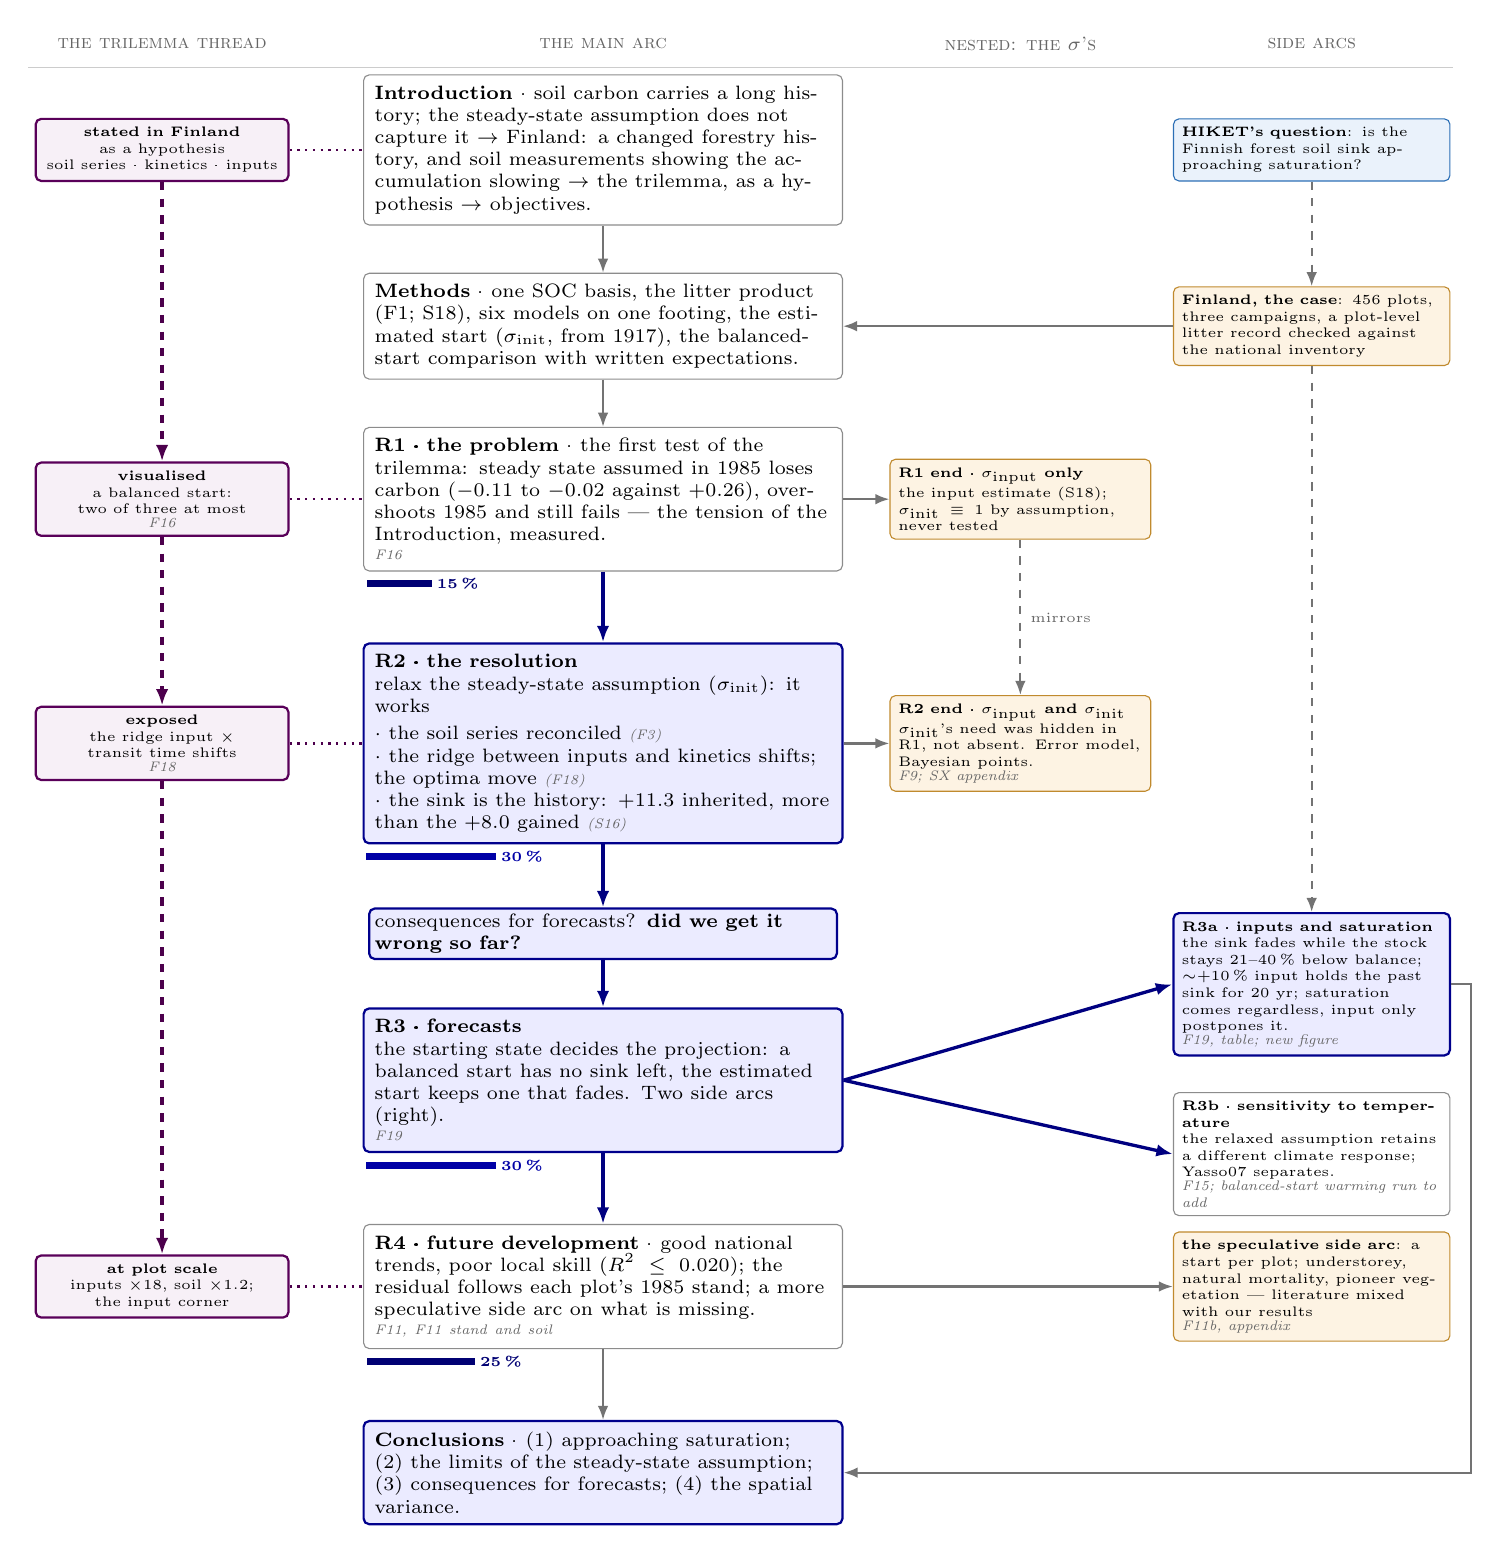
\begin{tikzpicture}[
  sp/.style={cl=58mm, inner sep=4pt},
  tm/.style={cl=30mm, thr, font=\tiny, align=center},
  sg/.style={cl=31mm, cav, align=left},
  sa/.style={cl=33mm, font=\tiny},
  lh/.style={font=\scriptsize\scshape, text=black!60},
  hook/.style={dotted, thick, violet!60!black}]
\coordinate (xT) at (0,0); \coordinate (xS) at (10.9,0); \coordinate (xF) at (14.6,0);
% --- lane headers ---
\node[lh] at (0, 1.35)    {the trilemma thread};
\node[lh] at (5.6, 1.35)  {the main arc};
\node[lh] at (10.9, 1.35) {nested: the $\sigma$'s};
\node[lh] at (14.6, 1.35) {side arcs};
\draw[black!20] (-1.7,1.05) -- (16.4,1.05);
% --- the main arc (spine) ---
\node[sp] (I) at (5.6, 0) {\textbf{Introduction} · soil carbon carries a long history; the steady-state
  assumption does not capture it $\to$ Finland: a changed forestry history, and soil measurements showing the
  accumulation slowing $\to$ the trilemma, as a hypothesis $\to$ objectives.};
\node[sp, below=6mm of I] (M) {\textbf{Methods} · one SOC basis, the litter product (F1; S18), six models on
  one footing, the estimated start ($\sigma_{\mathrm{init}}$, from 1917), the balanced-start comparison with
  written expectations.};
\node[sp, below=6mm of M] (R1) {\textbf{R1 · the problem} · the first test of the trilemma: steady state
  assumed in 1985 loses carbon ($-0.11$ to $-0.02$ against $+0.26$), overshoots 1985 and still fails --- the
  tension of the Introduction, measured. \ev{F16}};
\node[sp, key, below=9mm of R1] (R2) {\textbf{R2 · the resolution}\\
  relax the steady-state assumption ($\sigma_{\mathrm{init}}$): it works\\[2pt]
  $\cdot$ the soil series reconciled {\tiny\itshape\color{black!60}(F3)}\\
  $\cdot$ the ridge between inputs and kinetics shifts; the optima move {\tiny\itshape\color{black!60}(F18)}\\
  $\cdot$ the sink is the history: $+11.3$ inherited, more than the $+8.0$ gained {\tiny\itshape\color{black!60}(S16)}};
\node[sp, key, font=\scriptsize, inner sep=2pt, below=8mm of R2] (H) {consequences for forecasts? \textbf{did we
  get it wrong so far?}};
\node[sp, key, below=6mm of H] (R3) {\textbf{R3 · forecasts}\\the starting state decides the projection: a
  balanced start has no sink left, the estimated start keeps one that fades. Two side arcs (right).
  \ev{F19}};
\node[sp, below=9mm of R3] (R4) {\textbf{R4 · future development} · good national trends, poor local skill
  ($R^2 \le 0.020$); the residual follows each plot's 1985 stand; a more speculative side arc on what is
  missing. \ev{F11, F11 stand and soil}};
\node[sp, key, below=9mm of R4] (C) {\textbf{Conclusions} · (1) approaching saturation; (2) the limits of the
  steady-state assumption; (3) consequences for forecasts; (4) the spatial variance.};
\foreach \a/\b in {I/M, M/R1, R4/C} \draw[arr] (\a) -- (\b);
\draw[arrk] (R1) -- (R2); \draw[arrk] (R2) -- (H); \draw[arrk] (H) -- (R3); \draw[arrk] (R3) -- (R4);
% --- weights ---
\wbar{R1}{15} \wbar[blue!65!black]{R2}{30} \wbar[blue!65!black]{R3}{30} \wbar{R4}{25}
% --- the trilemma thread ---
\node[tm] (t0) at (xT |- I)  {\textbf{stated in Finland}\\as a hypothesis\\{\tiny soil series · kinetics · inputs}};
\node[tm] (t1) at (xT |- R1) {\textbf{visualised}\\a balanced start: two of three at most \ev{F16}};
\node[tm] (t2) at (xT |- R2) {\textbf{exposed}\\the ridge input $\times$ transit time shifts \ev{F18}};
\node[tm] (t3) at (xT |- R4) {\textbf{at plot scale}\\inputs $\times 18$, soil $\times 1.2$; the input corner};
\foreach \a/\b in {t0/t1, t1/t2, t2/t3} \draw[arrt] (\a) -- (\b);
\draw[hook] (t0) -- (I); \draw[hook] (t1) -- (R1); \draw[hook] (t2) -- (R2); \draw[hook] (t3) -- (R4);
% --- nested sigma side arm ---
\node[sg] (s1) at (xS |- R1) {\textbf{R1 end · $\sigma_{\mathrm{input}}$ only}\\the input estimate (S18);
  $\sigma_{\mathrm{init}} \equiv 1$ by assumption, never tested};
\node[sg] (s2) at (xS |- R2) {\textbf{R2 end · $\sigma_{\mathrm{input}}$ and $\sigma_{\mathrm{init}}$}\\
  $\sigma_{\mathrm{init}}$'s need was hidden in R1, not absent. Error model, Bayesian points.
  \ev{F9; SX appendix}};
\draw[arr] (R1) -- (s1); \draw[arr] (R2) -- (s2);
\draw[arr, dashed] (s1) -- node[right, font=\tiny, text=black!60] {mirrors} (s2);
% --- side arcs ---
\node[sa, draw=noterule, fill=notebg] (aim) at (xF |- I) {\textbf{HIKET's question}: is the Finnish forest
  soil sink approaching saturation?};
\node[sa, cav] (ft) at (xF |- M) {\textbf{Finland, the case}: 456 plots, three campaigns, a plot-level litter
  record checked against the national inventory};
\draw[arr] (ft.west) -- (M.east);
\node[cl=33mm, key, font=\tiny, anchor=south] (Ra) at ($(xF |- R3)+(0,0.3)$) {\textbf{R3a · inputs and
  saturation}\\the sink fades while the stock stays 21--40\,\% below balance; $\sim$+10\,\% input holds the
  past sink for 20~yr; saturation comes regardless, input only postpones it. \ev{F19, table; new figure}};
\node[cl=33mm, font=\tiny, anchor=north] (Rb) at ($(xF |- R3)+(0,-0.15)$) {\textbf{R3b · sensitivity to
  temperature}\\the relaxed assumption retains a different climate response; Yasso07 separates. \ev{F15;
  balanced-start warming run to add}};
\draw[arrk] (R3.east) -- (Ra.west); \draw[arrk] (R3.east) -- (Rb.west);
\node[sa, cav] (sp) at (xF |- R4) {\textbf{the speculative side arc}: a start per plot; understorey, natural
  mortality, pioneer vegetation --- literature mixed with our results \ev{F11b, appendix}};
\draw[arr] (R4.east) -- (sp.west);
\draw[arr, dashed] (aim) -- (ft); \draw[arr, dashed] (ft) -- (Ra);
\draw[arr] (Ra.east) -- ++(0.25,0) |- (C.east);
\end{tikzpicture}}
\end{center}}

% --- INTRODUCTION ---
\newcommand{\archIntro}{%
\begin{center}
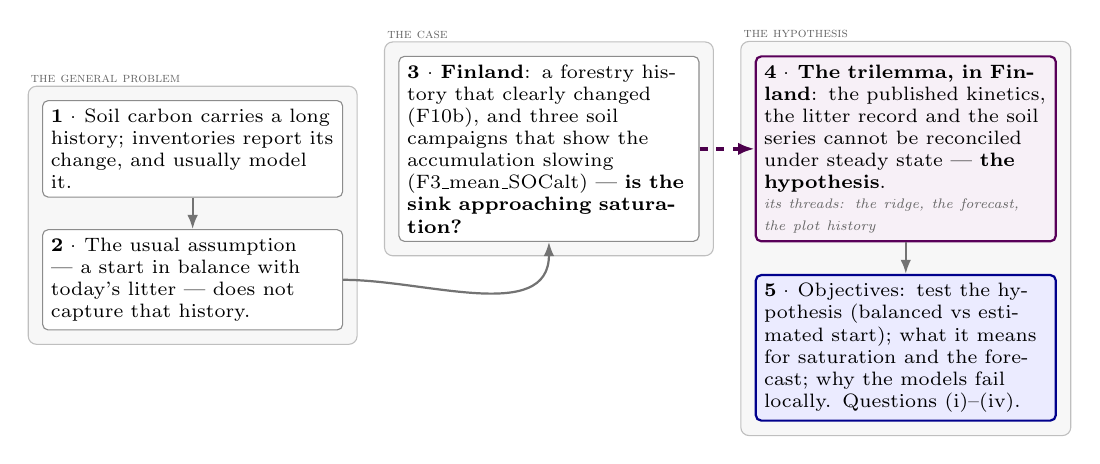
\begin{tikzpicture}[node distance=4mm]
\node[cl=36mm] (n1) {\textbf{1} · Soil carbon carries a long history; inventories report its change, and
  usually model it.};
\node[cl=36mm, below=of n1] (n2) {\textbf{2} · The usual assumption --- a start in balance with today's
  litter --- does not capture that history.};
\node[cl=36mm, right=7mm of n1] (n3) {\textbf{3} · \textbf{Finland}: a forestry history that clearly changed
  (F10b), and three soil campaigns that show the accumulation slowing (F3\_mean\_SOCalt) --- \textbf{is the sink
  approaching saturation?}};
\node[cl=36mm, thr, right=7mm of n3] (n4) {\textbf{4} · \textbf{The trilemma, in Finland}: the published
  kinetics, the litter record and the soil series cannot be reconciled under steady state --- \textbf{the
  hypothesis}. \ev{its threads: the ridge, the forecast, the plot history}};
\node[cl=36mm, key, below=of n4] (n5) {\textbf{5} · Objectives: test the hypothesis (balanced vs estimated
  start); what it means for saturation and the forecast; why the models fail locally. Questions (i)--(iv).};
\begin{scope}[on background layer]
  \node[grp, fit=(n1)(n2)] (g1) {}; \node[glab] at (g1.north west) {the general problem};
  \node[grp, fit=(n3)] (g2) {}; \node[glab] at (g2.north west) {the case};
  \node[grp, fit=(n4)(n5)] (g3) {}; \node[glab] at (g3.north west) {the hypothesis};
\end{scope}
\draw[arr] (n1) -- (n2); \draw[arr] (n4) -- (n5);
\draw[arr] (n2.east) to[out=0, in=-90] (n3.south);
\draw[arrt] (n3) -- (n4);
\end{tikzpicture}
\end{center}}

% --- THE TRILEMMA (Introduction 4; comes back in R2 and R4) ---
\newcommand{\archTrilemma}{%
\begin{center}
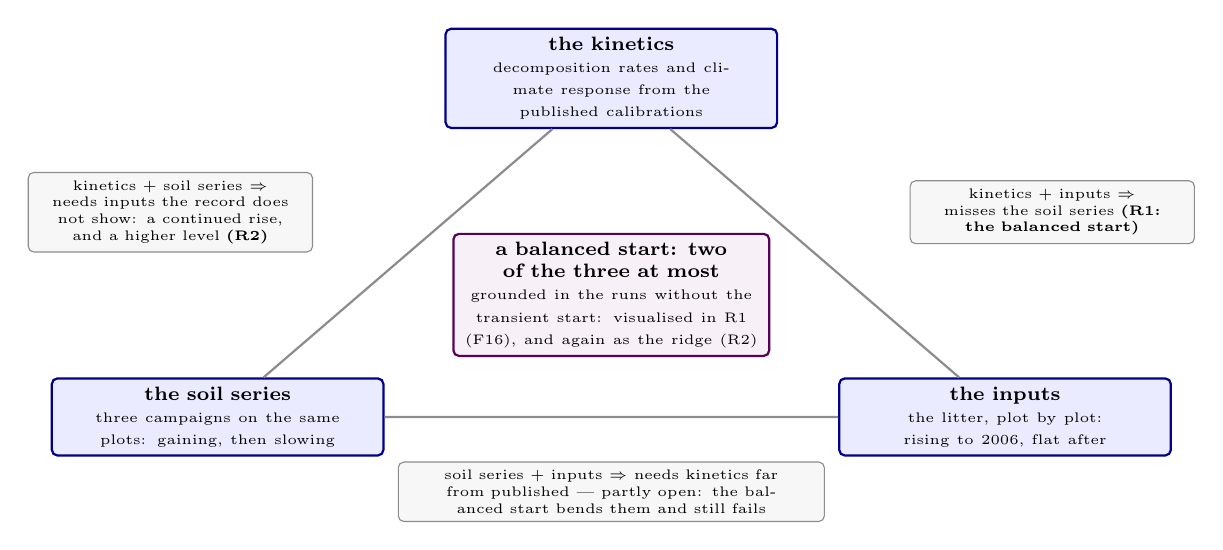
\begin{tikzpicture}[font=\scriptsize]
\node[cl=40mm, key, align=center] (K) at (0, 4.3) {\textbf{the kinetics}\\{\tiny decomposition rates and climate
  response from the published calibrations}};
\node[cl=40mm, key, align=center] (S) at (-5.0, 0) {\textbf{the soil series}\\{\tiny three campaigns on the
  same plots: gaining, then slowing}};
\node[cl=40mm, key, align=center] (L) at (5.0, 0) {\textbf{the inputs}\\{\tiny the litter, plot by plot:
  rising to 2006, flat after}};
\draw[thick, black!45] (K) -- (S) -- (L) -- (K);
\node[cl=34mm, font=\tiny, align=center, fill=black!3] at (-5.6, 2.6) {kinetics + soil series
  $\Rightarrow$ needs inputs the record does not show: a continued rise, and a higher level \textbf{(R2)}};
\node[cl=34mm, font=\tiny, align=center, fill=black!3] at (5.6, 2.6) {kinetics + inputs $\Rightarrow$ misses
  the soil series \textbf{(R1: the balanced start)}};
\node[cl=52mm, font=\tiny, align=center, fill=black!3] at (0, -0.95) {soil series + inputs $\Rightarrow$ needs
  kinetics far from published --- partly open: the balanced start bends them and still fails};
\node[cl=38mm, thr, align=center] at (0, 1.55) {\textbf{a balanced start: two of the three at most}\\
  {\tiny grounded in the runs without the transient start: visualised in R1 (F16), and again as the ridge
  (R2)}};
\end{tikzpicture}
\end{center}}

% --- METHODS ---
\newcommand{\archMethods}{%
\begin{center}
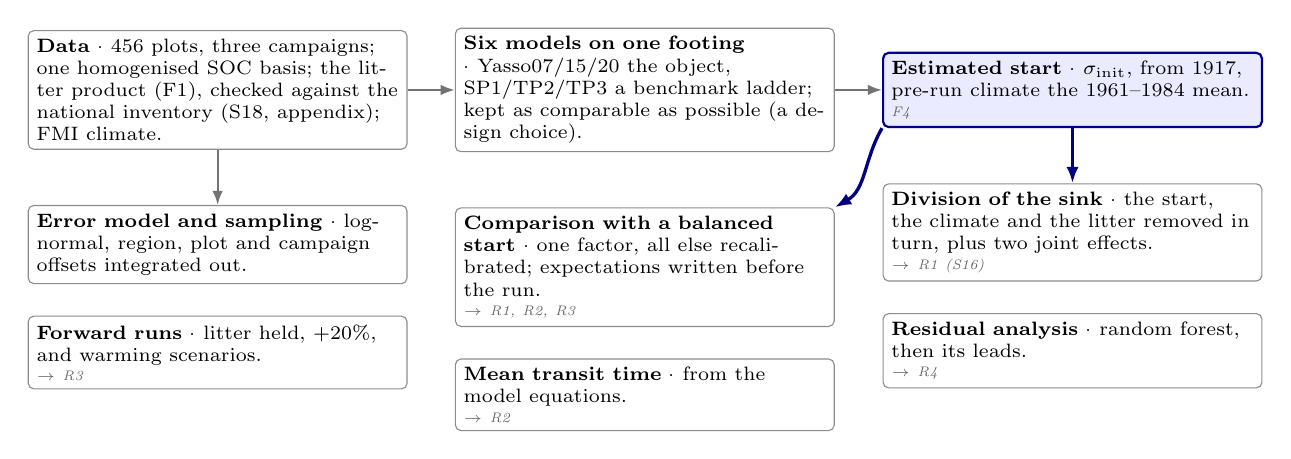
\begin{tikzpicture}[node distance=4mm and 6mm]
\node[cl=46mm] (d) {\textbf{Data} · 456 plots, three campaigns; one homogenised SOC basis; the litter
  product (F1), checked against the national inventory (S18, appendix); FMI climate.};
\node[cl=46mm, right=of d] (m) {\textbf{Six models on one footing} · Yasso07/15/20 the object, SP1/TP2/TP3 a
  benchmark ladder; kept as comparable as possible (a design choice).};
\node[cl=46mm, key, right=of m] (t) {\textbf{Estimated start} · $\sigma_{\mathrm{init}}$, from 1917,
  pre-run climate the 1961--1984 mean. \ev{F4}};
\node[cl=46mm, below=7mm of d] (e) {\textbf{Error model and sampling} · log-normal, region, plot and
  campaign offsets integrated out.};
\node[cl=46mm, below=7mm of m] (b) {\textbf{Comparison with a balanced start} · one factor, all else
  recalibrated; expectations written before the run. \ev{$\to$ R1, R2, R3}};
\node[cl=46mm, below=7mm of t] (a) {\textbf{Division of the sink} · the start, the climate and the litter
  removed in turn, plus two joint effects. \ev{$\to$ R1 (S16)}};
\node[cl=46mm, below=of e] (f) {\textbf{Forward runs} · litter held, $+20\%$, and warming scenarios.
  \ev{$\to$ R3}};
\node[cl=46mm, below=of b] (mt) {\textbf{Mean transit time} · from the model equations. \ev{$\to$ R2}};
\node[cl=46mm, below=of a] (r) {\textbf{Residual analysis} · random forest, then its leads. \ev{$\to$ R4}};
\draw[arr] (d) -- (m); \draw[arr] (m) -- (t); \draw[arrk] (t) -- (a);
\draw[arrk] (t.south west) to[out=-120, in=30] (b.north east); \draw[arr] (d) -- (e);
\end{tikzpicture}
\end{center}}

% --- R1 ---
\newcommand{\archRone}{%
\begin{center}
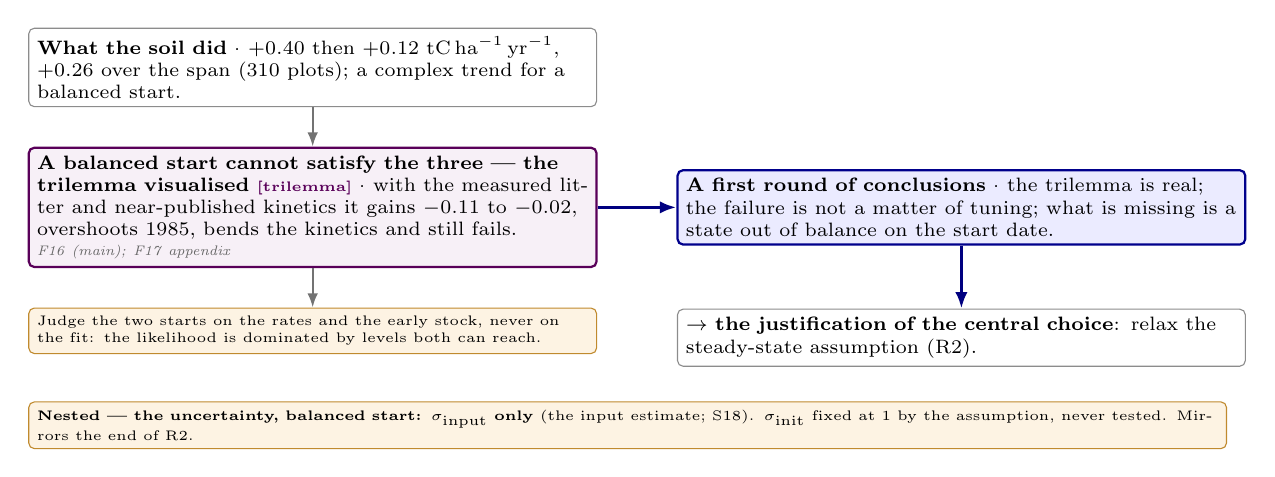
\begin{tikzpicture}[node distance=5mm and 8mm]
\node[cl=70mm] (o) {\textbf{What the soil did} · $+0.40$ then $+0.12$~tC\,ha$^{-1}$\,yr$^{-1}$, $+0.26$ over
  the span (310 plots); a complex trend for a balanced start.};
\node[cl=70mm, thr, below=of o] (A) {\textbf{A balanced start cannot satisfy the three --- the trilemma
  visualised} \TR\ · with the measured litter and near-published kinetics it gains $-0.11$ to $-0.02$,
  overshoots 1985, bends the kinetics and still fails. \ev{F16 (main); F17 appendix}};
\node[cl=70mm, cav, below=of A] (cv) {Judge the two starts on the rates and the early stock, never on the
  fit: the likelihood is dominated by levels both can reach.};
\node[cl=70mm, key, right=10mm of A] (c) {\textbf{A first round of conclusions} · the trilemma is real; the
  failure is not a matter of tuning; what is missing is a state out of balance on the start date.};
\node[cl=70mm, below=8mm of c] (j) {$\to$ \textbf{the justification of the central choice}: relax the
  steady-state assumption (R2).};
\node[cl=150mm, cav, below=6mm of cv.south west, anchor=north west] (u) {\textbf{Nested --- the uncertainty,
  balanced start: $\sigma_{\mathrm{input}}$ only} (the input estimate; S18). $\sigma_{\mathrm{init}}$ fixed at 1
  by the assumption, never tested. Mirrors the end of R2.};
\draw[arr] (o) -- (A); \draw[arr] (A) -- (cv); \draw[arrk] (A) -- (c); \draw[arrk] (c) -- (j);
\end{tikzpicture}
\end{center}}

% --- R2 ---
\newcommand{\archRtwo}{%
\begin{center}
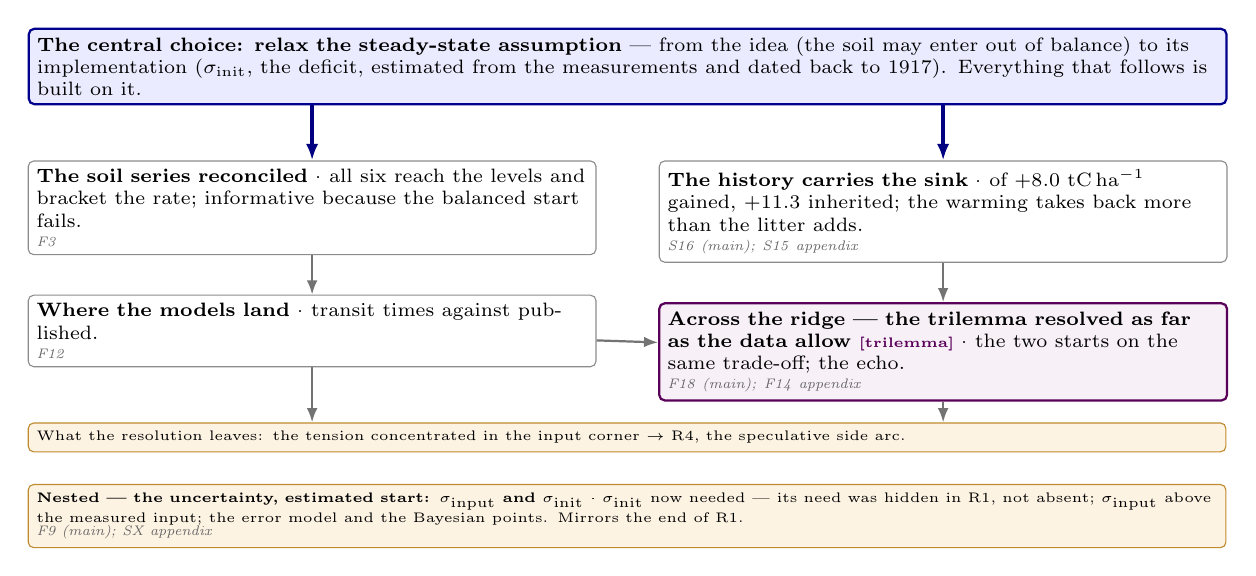
\begin{tikzpicture}[node distance=5mm and 8mm]
\node[cl=150mm, key] (ch) {\textbf{The central choice: relax the steady-state assumption} --- from the idea
  (the soil may enter out of balance) to its implementation ($\sigma_{\mathrm{init}}$, the deficit, estimated
  from the measurements and dated back to 1917). Everything that follows is built on it.};
\node[cl=70mm, below=7mm of ch.south west, anchor=north west] (B) {\textbf{The soil series reconciled} · all
  six reach the levels and bracket the rate; informative because the balanced start fails. \ev{F3}};
\node[cl=70mm, below=7mm of ch.south east, anchor=north east] (S) {\textbf{The history carries the sink} · of
  $+8.0$~tC\,ha$^{-1}$ gained, $+11.3$ inherited; the warming takes back more than the litter adds. \ev{S16 (main); S15 appendix}};
\node[cl=70mm, below=of B] (i) {\textbf{Where the models land} · transit times against published. \ev{F12}};
\node[cl=70mm, thr, below=of S] (r) {\textbf{Across the ridge --- the trilemma resolved as far as the data
  allow} \TR\ · the two starts on the same trade-off; the echo. \ev{F18 (main); F14 appendix}};
\node[cl=150mm, cav, below=7mm of i.south west, anchor=north west] (l) {What the resolution leaves: the tension
  concentrated in the input corner $\to$ R4, the speculative side arc.};
\node[cl=150mm, cav, below=4mm of l] (u) {\textbf{Nested --- the uncertainty, estimated start:
  $\sigma_{\mathrm{input}}$ and $\sigma_{\mathrm{init}}$} · $\sigma_{\mathrm{init}}$ now needed --- its need was
  hidden in R1, not absent; $\sigma_{\mathrm{input}}$ above the measured input; the error model and the Bayesian
  points. Mirrors the end of R1. \ev{F9 (main); SX appendix}};
\draw[arrk] (ch.south -| B.north) -- (B.north); \draw[arrk] (ch.south -| S.north) -- (S.north);
\draw[arr] (B) -- (i); \draw[arr] (S) -- (r); \draw[arr] (i) -- (r);
\draw[arr] (i.south) -- (i.south |- l.north); \draw[arr] (r.south) -- (r.south |- l.north);
\end{tikzpicture}
\end{center}}

% --- R3 ---
\newcommand{\archRthree}{%
\begin{center}
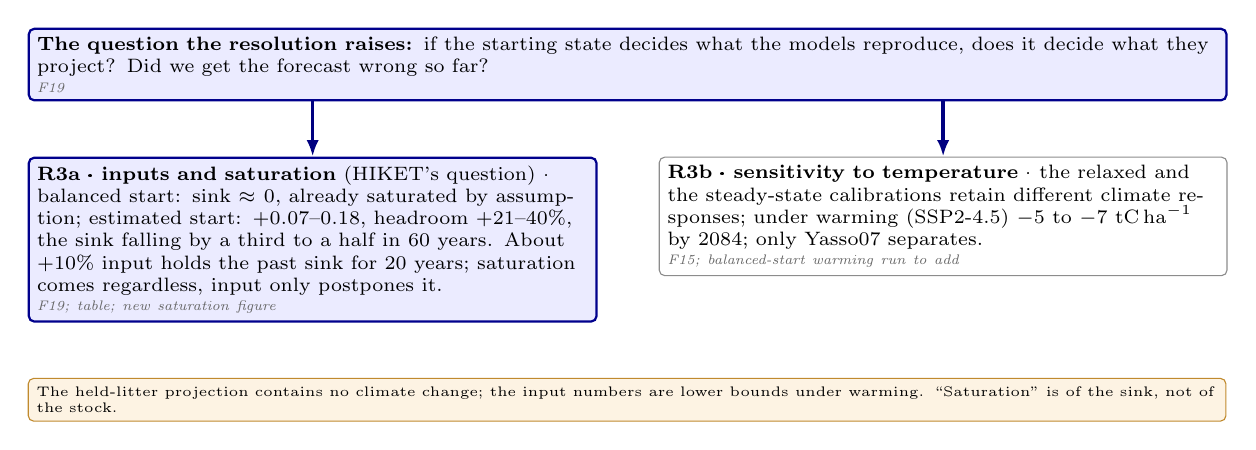
\begin{tikzpicture}[node distance=5mm and 8mm]
\node[cl=150mm, key] (q) {\textbf{The question the resolution raises:} if the starting state decides what the
  models reproduce, does it decide what they project? Did we get the forecast wrong so far? \ev{F19}};
\node[cl=70mm, key, below=7mm of q.south west, anchor=north west] (a) {\textbf{R3a · inputs and saturation}
  (HIKET's question) · balanced start: sink $\approx 0$, already saturated by assumption; estimated start:
  $+0.07$--$0.18$, headroom $+21$--$40\%$, the sink falling by a third to a half in 60 years. About $+10\%$
  input holds the past sink for 20 years; saturation comes regardless, input only postpones it.
  \ev{F19; table; new saturation figure}};
\node[cl=70mm, below=7mm of q.south east, anchor=north east] (b) {\textbf{R3b · sensitivity to temperature}
  · the relaxed and the steady-state calibrations retain different climate responses; under warming
  (SSP2-4.5) $-5$ to $-7$~tC\,ha$^{-1}$ by 2084; only Yasso07 separates. \ev{F15; balanced-start warming run to add}};
\node[cl=150mm, cav, below=7mm of a.south west, anchor=north west] (c) {The held-litter projection contains
  no climate change; the input numbers are lower bounds under warming. ``Saturation'' is of the sink, not of
  the stock.};
\draw[arrk] (q.south -| a.north) -- (a.north); \draw[arrk] (q.south -| b.north) -- (b.north);
\end{tikzpicture}
\end{center}}

% --- R4 ---
\newcommand{\archRfour}{%
\begin{center}
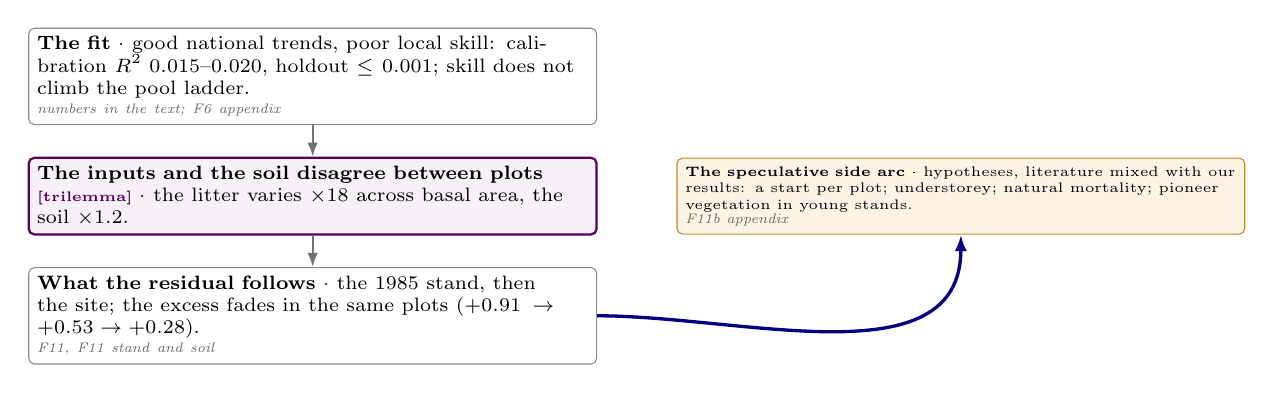
\begin{tikzpicture}[node distance=4mm and 8mm]
\node[cl=70mm] (f) {\textbf{The fit} · good national trends, poor local skill: calibration $R^2$
  $0.015$--$0.020$, holdout $\le 0.001$; skill does not climb the pool ladder. \ev{numbers in the text; F6 appendix}};
\node[cl=70mm, thr, below=of f] (g) {\textbf{The inputs and the soil disagree between plots} \TR\ · the
  litter varies $\times 18$ across basal area, the soil $\times 1.2$.};
\node[cl=70mm, below=of g] (s) {\textbf{What the residual follows} · the 1985 stand, then the site; the
  excess fades in the same plots ($+0.91 \to +0.53 \to +0.28$). \ev{F11, F11 stand and soil}};
\node[cl=70mm, cav, right=10mm of g] (e) {\textbf{The speculative side arc} · hypotheses, literature mixed with
  our results: a start per plot; understorey; natural mortality; pioneer vegetation in young stands.
  \ev{F11b appendix}};
\draw[arr] (f) -- (g); \draw[arr] (g) -- (s); \draw[arrk] (s.east) to[out=0, in=-90] (e.south);
\end{tikzpicture}
\end{center}}

% --- CONCLUSIONS ---
\newcommand{\archConcl}{%
\begin{center}
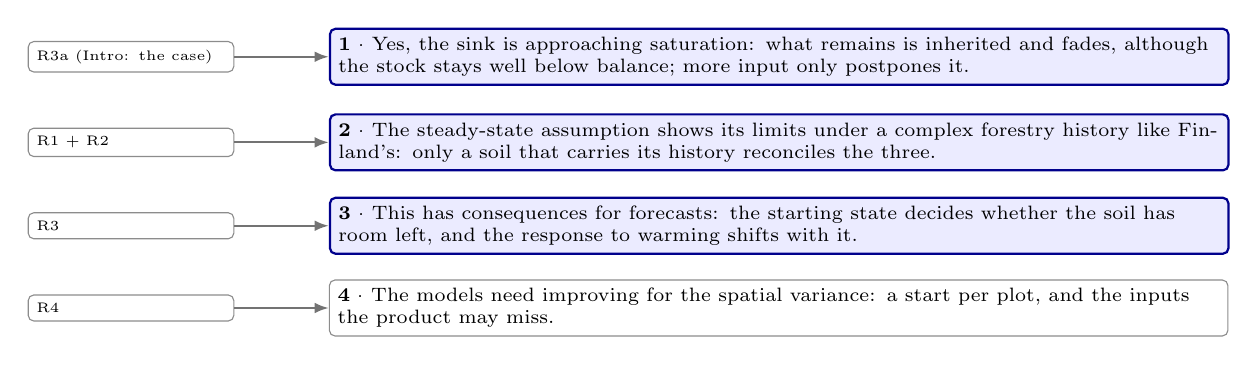
\begin{tikzpicture}[node distance=3mm]
\node[cl=24mm, font=\tiny] (p1) {R3a (Intro: the case)};
\node[cl=24mm, font=\tiny, below=7mm of p1] (p2) {R1 + R2};
\node[cl=24mm, font=\tiny, below=7mm of p2] (p3) {R3};
\node[cl=24mm, font=\tiny, below=7mm of p3] (p4) {R4};
\node[cl=112mm, key, right=12mm of p1] (c1) {\textbf{1} · Yes, the sink is approaching saturation: what remains
  is inherited and fades, although the stock stays well below balance; more input only postpones it.};
\node[cl=112mm, key, right=12mm of p2] (c2) {\textbf{2} · The steady-state assumption shows its limits under a
  complex forestry history like Finland's: only a soil that carries its history reconciles the three.};
\node[cl=112mm, key, right=12mm of p3] (c3) {\textbf{3} · This has consequences for forecasts: the starting
  state decides whether the soil has room left, and the response to warming shifts with it.};
\node[cl=112mm, right=12mm of p4] (c4) {\textbf{4} · The models need improving for the spatial variance: a start
  per plot, and the inputs the product may miss.};
\foreach \a/\b in {p1/c1, p2/c2, p3/c3, p4/c4} \draw[arr] (\a) -- (\b);
\end{tikzpicture}
\end{center}}

\title{\vspace{-1.4cm}\textbf{HIKET --- the storyline}\\[2pt]
\large a soil that carries its history: the trilemma of the balanced start, tested in Finland}
\author{}
\date{\small Version of \today. Numbers restated on 2026-10-13 on the recalibrated pair with the 1961--1984
pre-run climate: production \texttt{20261012\_1042*}; balanced start \texttt{20261012\_12*--13*}.}

\begin{document}\maketitle

\begin{note}
\textbf{How to read this.} A basis for the story discussion, not a draft. Each section opens with a strip
of the whole paper, its own place highlighted, and then its internal arc. In the diagrams: blue = the
section's payload; violet = a thread of the trilemma; amber fill = a caveat that travels with a claim.
Figures sit where they are used: captions say \emph{main text}, \textcolor{warnrule}{\textbf{appendix}} or
\textcolor{lorrule}{\textbf{not in your list: keep?}}. Green boxes are the questions still open.
\end{note}

\begin{ann}
\textbf{The decisions this storyline is built on (Lorenzo, 2026-10-12; story recomposed 2026-10-13 for the
discussion with Samuli and Aleksi).}
\begin{itemize}\itemsep0pt
  \item \textbf{General first, then the case.} Soil carbon carries a long history, and the usual assumption of
    steady state does not capture it. Then the particular: Finland, where the forestry history clearly
    changed and the soil has been measured, and where the measurements show the accumulation slowing ---
    HIKET's own question, \emph{is the sink approaching saturation?}
  \item \textbf{The trilemma is introduced in Finland, as a hypothesis.} The kinetics, the inputs and the soil
    series cannot be reconciled under the steady-state assumption: motivated in the Introduction, tested
    in the Results. Published kinetics are a source of information like the others.
  \item \textbf{R1 opens the Results with the first test of the trilemma}: the steady state assumed in 1985
    does not work. The tension, only hypothesised in the Introduction, becomes measured (F16).
  \item \textbf{R2 is the resolution}: the relaxed assumption works, and exposes the trilemma further --- the
    ridge between inputs and kinetics shifts in model space and the optima move (F3, F18). S16 closes R2:
    the sink is the history, which is also the bridge to the forecast.
  \item \textbf{R3 asks the question the resolution raises}: are there consequences for forecasts --- did we
    get it wrong so far? Two side arcs: \textbf{the sensitivity to temperature} under the relaxed assumption,
    and \textbf{the inputs}, central to HIKET --- are we approaching saturation under the more realistic
    assumption, how much input would push it forward in time, with the short digression that saturation
    comes regardless and can only be postponed.
  \item \textbf{R4 is future development}, the more speculative side arc: good trends, poor local skill; the
    residual analysis and its relationships; the hypotheses (understorey and pioneer vegetation missing),
    with literature mixed with our results. The separate Discussion section is folded into it.
  \item \textbf{The uncertainty stays a nested side arm} at the end of R1 ($\sinput$ only) and of R2 ($\sinput$
    and $\sinit$): $\sinit$'s need was hidden in R1 by the assumption, not absent.
  \item \textbf{Conclusions, in this order}: (1) yes, we are approaching saturation; (2) the steady-state
    assumption shows its limits under a complex forestry history like Finland's; (3) this has consequences
    for forecasts; (4) the models need improving for the spatial variance.
  \item \textbf{The story follows the discovery.} We started from a general question set by HIKET and found
    things on the way, so the opening does not mirror the conclusions one to one. It still closes the loop:
    the saturation question opens the paper (the case) and is answered first (conclusion 1); the limit of
    the assumption is the obstacle found on the way.
\end{itemize}
\end{ann}

% =====================================================================
\section*{The story on one page}
\addcontentsline{toc}{section}{The story on one page}

\paragraph{The general problem.} Soil carbon carries a long history. Its slowest pools adjust to a change in
their input over centuries, much longer than the few decades a unit of carbon spends in the soil on
average, so the soil of today still reflects the land use and the inputs of long before any model starts.
The usual assumption, a start in balance with the present litter, does not capture that history.

\paragraph{The case.} Finland: a forestry history that clearly changed --- slash-and-burn, grazing and
high-grading, the war decades, then a century of regrowth --- and soil carbon measured three times on the
same plots over four decades. The measurements show the soil gaining and the gain slowing. Is the forest
soil sink approaching saturation?

\paragraph{The hypothesis: a trilemma.} In Finland three sources of information are available on the same
ground: the published \emph{kinetics} of the inventory's own model family, the plot-level \emph{inputs}, and
the \emph{soil series}. Under the steady-state assumption they cannot be reconciled: a model started in
balance can satisfy two of them at most.

\paragraph{The test and the resolution.} Started in balance in 1985 and recalibrated, all six models lose
carbon over 1985--2024 against a measured gain. With the starting state estimated from the measurements and
dated back to 1917, they reach the measured accumulation, and the ridge between input and turnover shifts:
the optima move. The modelled sink is then the soil still catching up with its own history.

\paragraph{The consequences.} The starting state decides the forecast. A soil assumed balanced has no sink
left; a soil carrying its history keeps one, which fades: yes, the sink is approaching saturation, while the
stock stays well below balance. About a tenth more litter input would hold the sink of the past for twenty
years, postponing saturation rather than removing it, and the response to warming shifts with the
assumption.

\paragraph{Future development.} The models reproduce the national trend but not the differences between
plots. What they leave behind follows the history of each stand, and points to inputs no tree-based product
records: the understorey, natural mortality, the pioneer vegetation of young stands.

\paragraph{The arc of the whole paper.}
\archOverall

\begin{test}
\textbf{The weight budget, proposed for the recomposed story:} \textbf{R1} the problem $\sim$15\%;
\textbf{R2} the resolution $\sim$30\%; \textbf{R3} the forecasts and their two side arcs $\sim$30\%;
\textbf{R4} future development, with its speculative side arc $\sim$25\%. R3 grows because the saturation
question is conclusion 1.
\end{test}

% =====================================================================
\clearpage
\section*{The storyline schema}
\addcontentsline{toc}{section}{The storyline schema}
The whole paper on one page, in four lanes. \textbf{The main arc} runs down the middle: the Introduction
moves from the general problem to the Finnish case and the hypothesis, R1 tests it, R2 resolves it by
relaxing the steady-state assumption, and the resolution raises the question of R3 --- did we get the
forecast wrong? --- before R4 turns to what the models still miss. \textbf{The trilemma thread} (left, violet)
is stated in Finland as a hypothesis and comes back where it becomes visible: the failure of the balanced
start (F16), the shifting ridge (F18), and the plots. \textbf{The nested $\sigma$ side arm} closes R1 and R2.
\textbf{The side arcs} (right) hang off R3 --- inputs and saturation, the sensitivity to temperature --- and
off R4, the speculative arc on missing inputs. HIKET's saturation question opens the right lane and closes in
conclusion 1. Bars give the proposed weight of each section.

\archSchema

\clearpage
% =====================================================================
\section*{The figure plan}
\addcontentsline{toc}{section}{The figure plan}

\begin{center}\small
\begin{tabular}{llp{6.6cm}l}
\hline
where & figure & role & status \\
\hline
Introduction & F10b\_forest\_history & the case: a forestry history that changed & main (merge with the next?) \\
Introduction & F3\_mean\_SOCalt & the case: the measured soil, gaining and slowing & main \\
Methods & F1\_inputs & the litter series, one corner of the trilemma & main \\
Methods & \emph{S18} & litter: plot product vs national inventory, same scope & appendix \\
Methods & \emph{F2\_baseline} & one homogenised SOC basis & appendix? \\
Methods & F4\_initialization & how the estimated start is built & main \\
R1 & F16\_eqinit\_trajectories & the first test: the balanced start against the campaigns & main \\
R1 & \emph{F17} & the balanced start, rates by interval & appendix \\
R2 & F3\_mean\_soc & the relaxed assumption works & main \\
R2 & F18\_eqinit\_tradeoff & the ridge shifts, the optima move & main \\
R2 & S16\_attribution\_ensemble & the sink is the history --- the bridge to R3 & main \\
R2 & \emph{S15}, \emph{F12}, \emph{F14} & per model; transit times; the likelihood surface & appendix \\
R2 & \emph{F9}, \emph{SX} & the two auxiliary parameters (nested part) & appendix? \\
R3a & F19\_eqinit\_forecast & the forecast under the two assumptions: room left or not & main \\
R3a & \emph{table} & the input that would hold the sink & main \\
R3a & \emph{new} & saturation: held litter vs $+20\%$, the sink fading, saturation postponed & \textbf{to build} \\
R3b & F15\_forward\_arms & the response to warming, published vs calibrated & main \\
R3b & \emph{new} & the warming response under the balanced-start calibration & \textbf{to compute} \\
R4 & \emph{F6} & predicted vs measured on held-out plots ($R^2$ in the text) & appendix \\
R4 & F11\_rf\_heatmap & what the residual follows & main \\
R4 & F11\_stand\_and\_soil & the stand of 1985 and the soil & main \\
R4 & \emph{F11b}, \emph{harvest}, \emph{Rh vs age} & the speculative side arc & appendix \\
\hline
\end{tabular}
\end{center}

\begin{test}
\textbf{To decide:} (a) merge F10b and F3\_mean\_SOCalt into one Introduction figure (history above, the soil
below)? (b) R3b as framed needs the warming response of the \emph{balanced-start} calibration --- F15 compares
published and calibrated parameters, not the two assumptions; a cheap rerun of the forward experiment on the
balanced-start posteriors. (c) The saturation figure for R3a, from the forward runs already done. (d) About
13 main figures with the merges.
\end{test}

% =====================================================================
\section{Introduction}
\arch{1}{\archIntro}

\paragraph{1. Soil carbon carries a long history, and its change is usually modelled.} Inventories report
the annual change in the soil carbon stock, not the stock. A few countries measure it (Sweden, Germany);
most model it, Finland with Yasso07. The slow pools adjust over centuries, while the mean transit time is
decades (Sierra et al.\ 2018): a soil keeps the memory of its past inputs for far longer than its
turnover suggests.

\paragraph{2. The usual assumption does not capture it.} Models are started in balance with a constant
litter and climate --- the Finnish inventory, the nationwide Yasso07 evaluation, RothC, the land models ---
and the inventory justifies it in one sentence (``approximately ten years of simulation since spin-up is
enough to cancel out the effect of the spin-up level''). A balanced start responds to every change after
its start date, but it cannot carry a deficit that already existed on that date: the site's history is
replaced by an equilibrium with its present litter.

\paragraph{3. The case: Finland, and the question of saturation.} A forestry history that clearly changed:
slash-and-burn, grazing and high-grading, the war decades, then a century of regrowth ($+84\%$ growing stock)
(Liski et al.\ 2006; Peltoniemi et al.\ 2004, 2007 said this in the group's own words). And the soil measured:
three campaigns on the same plots, $64.5 \to 71.5 \to 73.6$~tC\,ha$^{-1}$, gaining and then slowing. The
measurements suggest that the forest soil sink is approaching saturation --- HIKET's question, and the one the
paper answers first. \FIGQ{F10b_forest_history} \FIGQ{F3_mean_SOCalt}
\begin{warn}
\textbf{Two cautions.} (a) The slowing rests on the 2006--2024 interval, the fragile one (its rate interval
includes zero): ``suggest'', not ``show''. (b) The reported Finnish soil term turned into a source from 2021,
once the litter input was recalculated; it can illustrate how a balanced start makes the soil term follow
the litter. Describe the method, never judge the inventory (Aleksi leads it and is a coauthor): \emph{the
reported soil term is, in both directions, the response of a modelled soil to a litter input that departs
from the level the soil was started in balance with.}
\end{warn}

\paragraph{4. The trilemma, in Finland --- the hypothesis.} A model of a soil's trajectory has three sources of
information to reconcile, and in Finland all three are measured on the same ground: the \emph{soil series}
(the three campaigns), the \emph{kinetics} (the published calibrations of the inventory's own model family),
and the \emph{inputs} (a litter record for every plot, Tupek et al., rising by about $45\%$ to 2006 and flat
after, which agrees with the national inventory on the scope they share). In a soil in balance, the stock is
the input times the transit time, so the three are tied together: a soil that keeps gaining carbon while its
litter has stopped rising cannot be in balance with that litter. \textbf{Hypothesis: under the steady-state
assumption the three cannot be reconciled} --- a balanced start satisfies two at most. The trilemma rests on
the balanced-start runs, which cannot appear in the Introduction; it is motivated here and tested at the
opening of the Results (R1, F16). Its threads come back later: the ridge between input and turnover (R2), the
forecast (R3), and the history of each plot (R4).
\archTrilemma

\paragraph{5. Objectives.} Test the hypothesis: the same six models, started in balance at the beginning of
the measurements and with the starting state estimated and dated back to 1917, on the same data. Then follow
the consequences to HIKET's question. Questions:
\begin{enumerate}\itemsep0pt
  \item[(i)] Can a model started in balance reconcile the soil series, the kinetics and the inputs, and does
    relaxing the assumption?
  \item[(ii)] Where does reconciling them place the models on the trade-off between litter input and
    transit time?
  \item[(iii)] Under the relaxed assumption, is the forest soil sink approaching saturation, how does it
    respond to warming, and how much additional litter input would postpone saturation?
  \item[(iv)] Why do the models reproduce the national trend but not the differences between plots?
\end{enumerate}
\begin{warn}
\textbf{Scope of the applied claim.} The projections describe the calibrated models on the study plots, per
hectare: the national inventory's term is not re-estimated, and the baseline projection holds the litter at
2024 and recycles the recent climate. The answer to (iii) is a statement about direction and sensitivity, not
a forecast of the reported numbers. National units need a sourced area and Aleksi's review.
\end{warn}

\begin{test}
\textbf{For the discussion.} (a) The forecast consequence is now a question the Results raise (R3), not a
claim of the Introduction; one sentence in paragraph 2 can still hint that a balanced start also decides
what the model says about the future. (b) Name the balanced-start comparison in the objectives (as above), or
only in the Methods?
\end{test}

% =====================================================================
\section{Materials and methods}
\arch{2}{\archMethods}

\paragraph{Data.} As written. The litter input, one corner of the trilemma, is introduced with F1; where it
is introduced, a short paragraph compares it with the national inventory's estimate (already in the draft):
on the shared scope (tree turnover and harvest residues) the two agree in the south, where most plots lie,
and neither rises after about 2006; the north differs, but holds only 50 of the 456 plots; the inventory
also carries natural mortality, which grows and which the product lacks. S18 in the appendix.
\FIG{F1_inputs} \FIGA{S18_litter_vs_inventory} \FIG{F2_baseline}

\paragraph{The estimated start.} As written, with the pre-run climate now the 1961--1984 mean, so that the
soil enters 1985 adjusted to the climate it had lived in. \FIG{F4_initialization}

\paragraph{The comparison with a balanced start.} The same six models, data, likelihood and priors, with the
start fixed at balance in 1985 (the 1985--1989 litter and the pre-run climate) and $\sinit$ removed;
everything else recalibrated. One factor. Stated as \emph{the steady-state assumption applied at the start
of the measurements}, the strongest fair version because the models are free to compensate, and explicitly
not as the inventory's procedure. The expectations were written down before the run.

\paragraph{The division of the sink.} Three runs and two joint effects of climate, in the words of the
appendix.

\begin{test}
\textbf{Say in the Methods that the expectations were written before the run, and that two failed} (the
balanced start overshoots the 1985 stock; its litter multiplier went down, not up)?
\end{test}

% =====================================================================
\section{Results and discussion}

\subsection*{\textsc{R1 --- the opening: the problem, tested the hard way}}
\addcontentsline{toc}{subsection}{R1 --- the opening: the problem, tested the hard way}
\begin{ann}
\textbf{Role (Lorenzo, 2026-10-12).} R1 is the opening, a better definition of the problem. We know the
conceptual problem of a balanced start, and we know the data hold a complex trend that could trouble it;
here we test it the hard way and reach a first round of conclusions. From R1 to R2 runs the justification
of the central choice.
\end{ann}
\arch{3}{\archRone}

\subsubsection{What the soil did}
\paragraph{} $+0.40$~tC\,ha$^{-1}$\,yr$^{-1}$ over the first interval, $+0.12$ over the second, $+0.26$ over
the span (310 plots, unweighted, true sampling years). The second interval is the fragile one (its interval
includes zero); the span is robust.

\subsubsection{A balanced start cannot satisfy the three --- the trilemma visualised}
\paragraph{The first result, and the moment the trilemma of the Introduction becomes visible.} Started in
balance in 1985 and recalibrated, all six
models lose carbon over 1985--2024, $-0.11$ to $-0.02$, against the observed $+0.26$. They rise with the litter to 2006
and give the rise back after it, and they start about $9$~tC\,ha$^{-1}$ above the first campaign ($73$--$76$ against
$64.5$), because a soil in balance with the 1985 litter holds more carbon than the soil held. Over
1985--2006 none reaches the observed rise ($+0.06$ to $+0.20$ against $+0.40$); over 2006--2024 all six lose carbon. F16 shows it against
the campaigns: the two starts differ mainly at the first campaign, and separate again in the projection.
\FIG{F16_eqinit_trajectories} \FIGA{F17_eqinit_rates}

\dparagraph{The trilemma, contextualised.} The text names it here: held to the measured litter and to
kinetics near the published ones, the balanced start gives up the soil series --- the corner of the triangle
the Introduction predicted. It is free to bend the kinetics and does
--- less input, faster and more temperature-sensitive decomposition (transit time $22$--$27 \to 17$--$24$~yr)
--- and still cannot produce the accumulation. How far the kinetics would have to move is the corner the
comparison leaves partly open.
\begin{warn}
\textbf{Do not judge the two starts by the fit.} The likelihood is dominated by the stock levels, which both
starts reach (log-likelihoods within $8$, the estimated start better in five of six); the rates and the early stock discriminate. Say so in two
sentences before a reader concludes the starts are equivalent.
\end{warn}
\begin{test}
\textbf{Close the third corner?} A balanced start with the rate priors widened would show how far the
kinetics must move to fit both series; one factor, six jobs. Or state it as a limitation.
\end{test}

\subsubsection{A first round of conclusions --- and the justification of the central choice}
\paragraph{} Three things are settled before anything else is built. (1) The trilemma is real on these data:
with the measured litter and near-published kinetics, a soil assumed balanced in 1985 cannot reproduce the
measured accumulation. (2) The failure survives the freedom to compensate, so it is not a matter of tuning.
(3) What the balanced start lacks is a state that is not in balance on the start date. \textbf{That is the
justification for the central choice of the paper}: to relax the steady-state assumption and estimate the
starting state from the measurements, which is what R2 does.

\subsubsection{Nested: the uncertainty, as the balanced start sees it --- $\sinput$ only}
\paragraph{The same side arm as at the end of R2, with one parameter.} The balanced start carries one auxiliary
uncertainty parameter, $\sinput$, which absorbs the uncertainty of the input estimate --- the point where the
data discussion (the litter product against the national inventory, S18) enters the calibration. In the
balanced start it relaxes (Yasso15 $1.54 \to 1.31$, TP2 $1.75 \to 1.60$), while the kinetics strain.
\textbf{$\sinit$ is not absent: it is fixed at $1$ by the steady-state assumption} --- a value never questioned
and never tested, only assumed. Implementation details here: the same error model and priors as R2, the fit
equivalence of the two starts (the likelihood dominated by levels) and why the comparison is made on the
rates.



% ---------------------------------------------------------------- R2
\subsection*{\textsc{R2 --- the resolution: relaxing the steady-state assumption}}
\addcontentsline{toc}{subsection}{R2 --- the resolution: relaxing the steady-state assumption}
\arch{4}{\archRtwo}
\begin{ann}
\textbf{Role (Lorenzo, 2026-10-12).} The main arc, carrying the most load. Relaxing the steady-state
assumption is the paper's own approach to the trilemma --- the proposed solution, and \emph{the central
choice}. It moves the models across the ridge in parameter space, and the trade-off translates according
to the new assumption. Everything that follows (the forecast, the plot analyses) is built on it, once it is
justified; its ramifications are examined, but the choice is the centre.
\end{ann}

\subsubsection{The central choice}
\paragraph{From the general idea to its implementation.} The idea: the soil may enter the observations out of
balance. The implementation: the start is estimated from the measurements and dated back to 1917, through
one quantity, $\sinit$, the deficit the soil carries --- the parameter the balanced start had fixed at $1$.
The same data, priors and likelihood. What $\sinit$ means, and what it costs, is in the nested part at the
end of R2.

\subsubsection{The estimated start reconciles the soil series}
\paragraph{} All six reach the three campaign levels. Over 1985--2024 they span $+0.05$ to $+0.30$ against
the observed $+0.26$, four of six inside its interval (SP1 $+0.05$, Yasso20 $+0.10$ below). Over 1985--2006
all six reach the observed rise; over 2006--2024 only TP2 and TP3 reach the observed $+0.12$, Yasso07 is near
zero ($-0.03$), and SP1, Yasso15 and Yasso20 lose carbon. \FIG{F3_mean_soc}

\dparagraph{Bracketing is informative because it is not automatic.} Matching the rate would mean little if
any calibration on the same data could do it. The balanced start, calibrated on the same measurements with
one degree of freedom fewer, fails in every model.

\subsubsection{And the modelled sink is the history}
\paragraph{The division of the sink.} Six-model average, 1985--2024: of $+8.0$~tC\,ha$^{-1}$ gained, the
deficit inherited from before 1985 carries $+11.3$; the litter change since 1985 adds $+8.9$; the warming
since the 1961--1984 reference removes $-12.2$. The inherited part exceeds the whole sink in all six models. \FIG{S16_attribution_ensemble_smooth10} \FIGA{S15_attribution_by_model_smooth10}

\dparagraph{Necessary, and dominant.} The balanced start shows that the history is \emph{necessary} --- with
everything else free, the models cannot do without it. The division shows how much it \emph{weighs} --- more
than the whole sink, because the warming takes back more than the litter rise adds. The second answers the
objection to the first (``the inherited part is large only because the calibration chose a low $\sinit$''):
the data demand the deficit. \textbf{And it is the bridge to R3}: a sink that is the history is a sink that
fades --- the mechanism of the saturation the forecast will show.
\begin{warn}
\textbf{The numbers moved} with the 1961--1984 pre-run climate (2026-10-13), but not as expected: the inherited
part \emph{grew} ($+9.3 \to +11.3$), the climate part grew more ($-7.5 \to -12.2$, all warming since the colder
reference now counts), and the total fell ($+10.5 \to +8.0$). The robust statement is the ordering --- the
sink inherited; litter and warming of the same order and opposite sign. The size of the climate part
depends on the reference climate; say so.
\end{warn}
\begin{test}
\textbf{S16 in three parts or five terms} (the two joint effects of climate as hatched bands)?
\end{test}



\subsubsection{Where the models land: shorter transit times than published}
\paragraph{} Calibrated against published: Yasso07 and Yasso15 turn over faster, Yasso20 sits on its published
value. \FIG{F12_mrt_yasso}

\subsubsection{Across the ridge --- the trilemma resolved as far as the data allow}
\paragraph{} The soil fixes the product of input and transit time, and the posteriors ride that trade-off.
The two starts land at different places on it: in five of the six models the balanced start sits at less
input and faster turnover (SP1, a single slow pool, barely moves). \FIG{F18_eqinit_tradeoff}
\FIGA{F14_mrt_ridge}

\dparagraph{The echo, in parameter space.} \textbf{The triangle comes back once more}, after F16 showed it
in the trajectories. The
soil series is the ridge; the measured input (the dotted line) and the published kinetics sit off it; a
balanced start can stand on at most two of the three, and the estimated start, carrying the history,
stands somewhere else on the same ridge. Relaxing the assumption moves the models across it, and the
trade-off translates according to the new assumption. The text should say it in one or two sentences ---
after all the work, the trilemma is visible --- without redrawing the figure.

\dparagraph{What the resolution leaves.} The tension is not removed but concentrated in one corner: the soil
series is met and the kinetics stay near the published values (Yasso20 on its own, Yasso07 and Yasso15
faster), while the input the models need stays above what the product supplies. That remaining gap is the
thread to R4 and its side arc on the inputs the product may miss.

\subsubsection{Nested: the uncertainty, as the estimated start sees it --- $\sinput$ and $\sinit$}
\paragraph{The same side arm as at the end of R1, now with two parameters.} $\sinit$ becomes needed, and
\textbf{that need was there before}: in R1 it was hidden by forcing the steady-state assumption, which fixes it
at $1$. R2 may look more uncertain, but it only makes explicit a quantity R1 assumed without testing. The two
auxiliary parameters share a width by design.
\begin{itemize}\itemsep0pt
  \item \textbf{$\sinput$} --- more input than measured: effective flux $3.22$--$4.40$ against $2.511$, inside the
    envelope of boreal production, set by the likelihood rather than the prior (the posterior stays above the
    prior centre whichever anchor is used). The national inventory's full estimate is $1.08$--$1.26\times$ the
    product on the southern plots, bracketing the understorey-corrected anchor ($1.21$) and below the
    posteriors ($1.28$--$1.75$); SX sets it against independent estimates.
  \item \textbf{$\sinit$} --- the deficit the data demand: $0.45$--$0.56$ in five of six models (SP1 $0.78$), lower than the
    growing-stock record implies ($\sim 0.90$), so read as an \emph{effective starting deficit of the soil}
    (slash-and-burn, raking, heavy cutting) rather than a ratio of litter inputs. It carries the forecast:
    headroom correlates with it at $-0.76$ to $-0.97$ (R3).
  \item \textbf{The implementation, and its advantages}: the error model (region, plot and campaign offsets
    integrated out, a declared total of $0.800$), what it buys (an honest number of independent observations,
    $221$), and the Bayesian points --- priors as information, homogenised across models; the posterior
    against the prior.
\end{itemize}
\FIG{F9_auxiliary_sigmas} \FIGA{SX_input_vs_literature}
\begin{warn}
\textbf{The direction depends on the comparator, so the title names none.} Against the published parameters
the calibration has faster turnover (Yasso07, Yasso15); against the balanced start, slower. ``Displaces
along'' covers both; never add a direction.
\end{warn}

% ---------------------------------------------------------------- R3
\subsection*{\textsc{R3 --- consequences for forecasts: did we get it wrong?}}
\addcontentsline{toc}{subsection}{R3 --- consequences for forecasts: did we get it wrong?}
\paragraph{The question the resolution raises.} If the starting state decides what the models reproduce, it may
decide what they project: did we get the forecast wrong so far? Tested on the same models, now projected
forward, with two side arcs: the inputs and saturation --- HIKET's question --- and the sensitivity to
temperature. Within the scope declared in the objectives.
\arch{5}{\archRthree}

\subsubsection{The starting state decides the forecast}
\paragraph{} Projected over 2025--2044 with the litter held at 2024 and the recent climate recycled, the
balanced start gives a sink of $-0.12$ to $+0.02$~tC\,ha$^{-1}$\,yr$^{-1}$ and a headroom of $-8$ to $+9\%$:
a soil assumed balanced is saturated by assumption. The estimated start gives $+0.07$ to $+0.18$ and
$+21$ to $+40\%$ (SP1 $\approx 0$) --- the disequilibrium Liski et al.\ (2006) found by another route
($+38\%$). S16 explains it: the sink the models carry is the history, and the history fades.
\FIG{F19_eqinit_forecast}

\subsubsection{Side arc a: inputs and saturation --- are we approaching it?}
\paragraph{Yes, and the qualifier matters.} Under the relaxed assumption the sink falls by a third to a half
within 60 years, while the stock stays 21--40\% below balance: the \emph{sink} saturates long before the
\emph{stock}, because the fast pools approach balance first and the remaining distance lies in the slow pool.
Saturation of the sink, not of the stock.

\dparagraph{How much input would push saturation forward in time?} The models are linear in their input, so
the projections with the litter held and with $+20\%$ answer it exactly for any target sink
(\texttt{doublechecks/input\_to\_hold\_sink.R}):
\begin{center}\small
\begin{tabular}{llccccc}
\hline
target sink & window & Yasso07 & Yasso15 & Yasso20 & TP2 / TP3 & SP1 \\
\hline
observed 1985--2024 ($+0.26$) & 10 yr & $+8\%$ & $+7\%$ & $+5\%$ & $+5$ / $+5\%$ & $+11\%$ \\
 & 20 yr & $\mathbf{+11\%}$ & $\mathbf{+10\%}$ & $\mathbf{+11\%}$ & $+7$ / $+6\%$ & $+13\%$ \\
each model's own 1985--2024 & 20 yr & $+9\%$ & $+7\%$ & $+3\%$ & $+10$ / $+10\%$ & $+4\%$ \\
observed 2006--2024 ($+0.12$) & 20 yr & $+2\%$ & $+2\%$ & $+3\%$ & $-5$ / $-5\%$ & $+6\%$ \\
\hline
\end{tabular}
\end{center}
About a tenth more input, sustained, holds the long-term sink for twenty years ($0.4$--$0.5$~tC\,ha$^{-1}$\,yr$^{-1}$
of effective input in Yasso; each $+10\%$ buys $0.15$--$0.24$~tC\,ha$^{-1}$\,yr$^{-1}$ of sink).

\dparagraph{A short digression: saturation comes regardless.} A higher input raises the eventual balance, so the
soil gains again, but the new sink fades in the same way: with $+20\%$ from 2025 the versions of Yasso realise
about half of the eventual gain within 60 years, and the gain lasts only while the input does. Input postpones
saturation; it does not remove it. \textbf{A figure to build} from the forward runs already done: held litter
against $+20\%$, the sink fading in both.
\begin{warn}
\textbf{Lower bounds:} no further warming is in these projections. The required input depends on both the
starting state (the baseline sink) and the transit time (the gain per unit of input).
\end{warn}
\begin{test}
\textbf{Which target}, the observed long-term rate, the recent one, or each model's own? A warming-corrected
column for Yasso? National units (Mt\,CO$_2$\,yr$^{-1}$) need a sourced area and Aleksi's eye.
\end{test}

\subsubsection{Side arc b: the sensitivity to temperature}
\paragraph{} Relaxing the assumption changes the kinetics the calibration retains: the balanced-start
calibration settles at faster and more temperature-sensitive decomposition (R1). Under warming to SSP2-4.5
the stock falls by $5$--$7$~tC\,ha$^{-1}$ by 2084 in all three Yasso versions; only Yasso07 separates the
published and calibrated parameters ($-2.22$~tC\,ha$^{-1}$), because its single climate modifier ties turnover
to temperature sensitivity. For the inventory, which runs Yasso07, that is the applied point.
\FIG{F15_forward_arms}
\begin{test}
\textbf{The comparison this arc needs is not yet computed.} F15 compares the published and the calibrated
parameters, both with a transient start; the arc as framed compares the two \emph{assumptions}. A rerun of
the forward experiment on the balanced-start posteriors would give the warming response with and without the
history --- cheap, no new calibration.
\end{test}

% ---------------------------------------------------------------- R4
\subsection*{\textsc{R4 --- future development: why the models fail locally}}
\addcontentsline{toc}{subsection}{R4 --- future development: why the models fail locally}
\arch{6}{\archRfour}

\subsubsection{Good trends, poor local skill}
\paragraph{} Calibration $R^2$ $0.015$--$0.020$, holdout $R^2 \le 0.001$; skill does not climb the pool ladder.
The models reproduce the national trend and almost none of the differences between plots. Numbers in the
text; F6 in the appendix. \FIGA{F6_obs_vs_pred_holdout}

\subsubsection{The inputs and the soil disagree between plots}
\paragraph{The trilemma at plot scale.} The litter product varies about $\times 18$ across the basal-area range;
the soil about $\times 1.2$. A soil in balance with its litter would follow it --- the inputs corner of the
trilemma seen plot by plot, in one sentence.

\subsubsection{What the residual follows: each plot carries its own history}
\paragraph{} The residual follows the 1985 stand, then the site (F11 $\to$ F11 stand and soil). In the same
plots it fades over the three campaigns ($+0.91 \to +0.53 \to +0.28$ for sparse 1985 stands): the signature of
a wrong starting state, not of a missing input. One national pre-run shape cannot carry each stand's history.
\FIG{F11_rf_heatmap} \FIG{F11_stand_and_soil}

\subsubsection{The speculative side arc: what the models miss}
\paragraph{Hypotheses, with the literature mixed with our results.}
\begin{enumerate}\itemsep0pt
  \item \textbf{A starting state per plot.} The plot-level error fades at about the models' turnover pace: a
    start built from each plot's own history (the last regeneration cut dated from the 1985 stand age) is the
    natural next step. The excess lives in stands young in 1985. \FIGA{F11b_time_since_cut}
  \item \textbf{Understorey.} Field-layer cover in 2023 (438 of 456 plots) adds a little after basal area;
    the plot-level understorey litter gives (J+u)/J $\approx 1.13$, below the posteriors.
  \item \textbf{Natural mortality} --- quantified in the national inventory, $0.1$--$0.16$~tC\,ha$^{-1}$\,yr$^{-1}$
    by now in the south, absent from the product; roots and rhizodeposition; mycorrhizal fungi; fine-root
    lifespan (pointing the other way). A set that brackets the input gap, never a sum that matches it.
  \item \textbf{Pioneer vegetation, where the two meet.} The excess carbon of the stands young in 1985 was
    built during early stand development, either inherited or supplied by vegetation no tree-based product
    records; the data do not separate the two. Lauri Mehtätalo (LUKE) to be cited \gapnote{which work}.
  \item \textbf{The site, briefly.} Fertility, texture and stones explain a further tenth of the residual
    \gapnote{check whether the stone effect is partly the stone correction of the observed stocks}.
\end{enumerate}

% =====================================================================
\section{Conclusions}
\arch{7}{\archConcl}

\paragraph{1. Yes, we are approaching saturation.} Under the relaxed assumption the remaining sink is
inherited and fades, by a third to a half within 60 years, although the stock stays 21--40\% below balance:
the sink saturates, not the stock. More input postpones saturation --- about a tenth more holds the past sink
for twenty years --- but does not remove it.
\paragraph{2. The steady-state assumption shows its limits under a complex forestry history like Finland's.}
Started in balance, the models cannot reconcile the soil series, the kinetics and the inputs; carrying the
history, they can, as far as the data allow, and the tension concentrates in the input corner.
\paragraph{3. This has consequences for forecasts.} The starting state decides whether the soil has room
left: a soil assumed balanced has none, one that carries its history keeps a fading sink. The response to
warming shifts with the assumption where turnover and temperature sensitivity are tied (Yasso07).
\paragraph{4. The models need improving for the spatial variance.} They reproduce the national trend but not
the plots: a starting state per plot, and the inputs no tree-based product records.

% =====================================================================
\section*{Open questions collected}
\addcontentsline{toc}{section}{Open questions collected}
\begin{enumerate}\itemsep0pt
  \item The weight budget for the recomposed story (15 / 30 / 30 / 25).
  \item Merge F10b and F3\_mean\_SOCalt into one Introduction figure.
  \item The 2021 source as an illustration in the Finnish case: keep, soften or move.
  \item ``Approaching saturation'': of the sink, not the stock; and the observed slowing rests on the fragile
    interval --- say ``suggest'' in the Introduction.
  \item The balanced-start comparison named in the objectives, or only in the Methods.
  \item The written expectations and the two that failed, in the Methods.
  \item R3b: compute the warming response under the balanced-start calibration.
  \item R3a: build the saturation figure (held litter vs $+20\%$).
  \item S16 in three parts or five terms; the size of its climate part depends on the reference climate.
  \item The target sink in the input table; a warming-corrected column; national units.
  \item Eventual: a recalibrated decomposition (each run its own calibration --- a comparison between
    assumptions only).
\end{enumerate}

\end{document}
